\documentclass[%
crop,
convert={outext=.svg,command=\unexpanded{pdf2svg \infile\space\outfile}},
multi=false,
% class=scrartcl,
fontsize=20pt]{standalone}
%\usetikzlibrary{...}% tikz package already loaded by 'tikz' option

\usepackage[dvipsnames]{xcolor}
\usepackage{tikz}
\usetikzlibrary{arrows.meta,graphs,decorations.pathmorphing,backgrounds,positioning,fit,
  petri,shapes,calc,matrix,trees,shadows,shapes.symbols}
\tikzset{
  pre/.style={<-,shorten <=1pt,>={Stealth[round]},semithick},
  post/.style={->,shorten >=1pt,>={Stealth[round]},semithick},
  bidir/.style={<->,shorten <=1pt,>={Stealth[round]},semithick},
}


\usepackage{ifthen}         % Conditional processing in tex


\usepackage[margin=10pt,font=small,labelfont=bf,labelsep=colon]{caption}

\usepackage{subcaption} % to deal with subtables and subfigures


\usepackage{ebgaramond}



\makeatletter
\begin{document}



\begin{figure}[htp]
  \centering
  \begin{subfigure}[t]{0.4\textwidth}
    \centering
    \adjustbox{scale=0.7}{
    } 
    \caption{Mnesia replica states can diverge depending on the ordering of delivery of operations.
    The purple operations are causally concurrent.}
  \end{subfigure}
  \hfill
  \begin{subfigure}[t]{0.57\textwidth}
    \centering
    \adjustbox{scale=0.7}{
    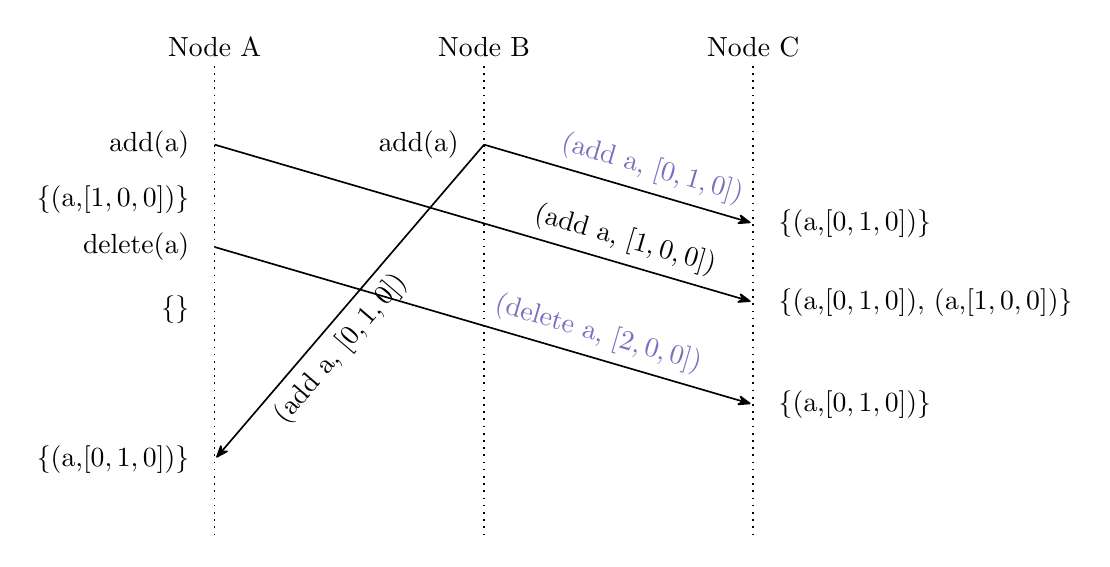
\begin{tikzpicture}[
      timeline/.style={semithick,dotted},
      commentl/.style={align=right},
      commentr/.style={commentl, align=left},]
      \node[] (n1) { Node A};
      \node[right=2cm of n1] (n2) { Node B};
      \node[right=2cm of n2] (n3) { Node C};
      
      \draw[post] ([yshift=-1cm]n2.south) coordinate (n2add) -- ([yshift=-4cm]n2add-|n1) 
        coordinate (n1addn2) node[pos=.6, sloped, auto, swap] {(add a, \([0,1,0]\))};
      \draw[post] (n2add) -- ([yshift=-1cm]n2add-|n3) 
        coordinate (n3addn2) node[pos=.6, above, sloped] 
        {\textcolor{Periwinkle}{(add a, \([0,1,0]\))}};
      \draw[post] ([yshift=-1cm]n1.south) coordinate (n1add) -- ([yshift=-2cm]n1add-|n3)
        coordinate (n3addn1) node[pos=.6, above, sloped,near end] {(add a, \([1,0,0]\))};
      \draw[post] ([yshift=-1.3cm]n1add) coordinate (n1rmv) -- ([yshift=-2cm]n1rmv-|n3)
        coordinate (n3rmvn1) node[pos=.7, above, sloped] 
        {\textcolor{Periwinkle}{(delete a, \([2,0,0]\))}};
      
      \draw[timeline] (n1) -- ($ (n1addn2) + (0, -1cm) $);
      \draw[timeline] (n2) -- ($ (n2|-n1addn2) + (0, -1cm) $);
      \draw[timeline] (n3) -- ($ (n3|-n1addn2) + (0,-1cm) $);
      
      \node[left=2mm of n1add, commentl] {add(a)};
      \node[below left=0.4cm and 2mm of n1add, commentl] {\{(a,\([1,0,0]\))\}};
      \node[left=2mm of n1rmv, commentl] {delete(a)};
      \node[below left=0.5cm and 2mm of n1rmv, commentl] {\{\}};
      \node[left=2mm of n1addn2, commentl] {\{(a,\([0,1,0]\))\}};
      \node[left=2mm of n2add, commentl] {add(a)};

      \node[right=2mm of n3addn2, commentr]  {\{(a,\([0,1,0]\))\}};
      \node[right=2mm of n3addn1, commentr]  {\{(a,\([0,1,0]\)), (a,\([1,0,0]\))\}};
      \node[right=2mm of n3rmvn1, commentr]  {\{(a,\([0,1,0]\))\}};
      \end{tikzpicture}
    } 
    \caption{Hypermnesia attaches vector timestamps to each message and stores them 
    along with actual elements in the set for conflict resolution.}
  \end{subfigure}
\end{figure}






\end{document}